\documentclass[conference]{IEEEtran}
\usepackage{graphicx}
\usepackage{amsmath}

\graphicspath{{./gambar/}}

\title{Analisis kekuatan Sinyal Menggunakan inSSIDer}

\author{Kevin Antony K\IEEEauthorrefmark{1}, Maranti Nainggolan\IEEEauthorrefmark{2}\\
\textit{Fakultas Teknologi Informasi}\\
\textit{Teknik Komputer}\\
\textit{Institut Teknologi Batam}\\
Batam, Indonesia\\
Email: \{\IEEEauthorrefmark{1}1922003, \IEEEauthorrefmark{2}1922023\}@student.iteba.ac.id}

\begin{document}
\maketitle

\begin{abstract} 
        Kemajuan teknologi informasi pada saat ini
terus berkembang seiring dengan kebutuhan manusia yang
menginginkan kemudahan, kecepatan, dan keakuratan dalam
memperoleh informasi. Oleh karena itu kemajuan teknologi
informasi di bidang transmisi pada saat ini yang berkembang
selain fiber optic ialah penggunaan perangkat wireless. Perangkat
wireless ini memungkinkan adanya hubungan para pengguna
informasi dalam melakukan aktivitasnya.
\end{abstract}  


\begin{IEEEkeywords}
Access Point, InSSIDer, SSID, Wi-Fi.
\end{IEEEkeywords}

\section{Introduction}
Teknologi Wifi atau yang dikenal dengan wireless LAN(WLAN) telah banyak diimplemantasikan 
oleh masyarakat baik didalam maupun diluar negeri.Selain untuk aplikasi privat,WLAN 
juga banyak digunakan untuk aplikasi public(hospot).\

\vspace{0.2cm}

WLAN merupakan jaringan yang tidak tampak karena
merupakan gelombang radio. Terutama bila frekuensinya terlalu
berdekatan, atau hilang oleh daya gelombang radio yang
lebih besar sehingga jaringan yang kita buat menjadi tidak
efisien. Untuk itu diperlukan suatu software yang dapat digunakan
untuk mencari informasi jaringan WLAN pada suatu
area lebih spesifik dari scan biasa. Salah satu software yang
dapat digunakan adalah inSSIDer~. \cite{b5}

\vspace{0.2cm}

InSSIDer merupakan software Wi-Fi scanner yang dapat
mengidentifikasi SSID, RSSI (Received Signal Strength Indicator),
security, dan pengaturan yang ada pada AP. Software
ini dikembangkan oleh MetaGeek, LLC dan lain lain.Berikut beberapa Tipe-tipe Wireless Network.\

1.Wireless Personal Area Network (WPAN)
WPAN (Wireless Personal Area Network) adalah sebuah bentuk komunikasi wireless yang terbatas hanya pada jarak pendek dan umumnya hanya terbatas untuk dua buah perangkat elektronik.
\vspace{5pt}

2.Wireless Wide Area Network (WWAN)
WWAN adalah sebuah bentuk komunikasi nirkabel yang memiliki area sangat luas, antara lain untuk penggunaan selular seperti 2G, 3G, 4G, dan lain sebagainya
\vspace{5pt}

3.Wireless Local Area Network (WLAN)
WLAN (Wireless Local Area Network) adalah sebuah bentuk komunikasi nirkabel yang memiliki area terbatas seperti dalam suatu ruangan ataupun sebuah gedung. WLAN memiliki standar komunikasi yang diatur oleh sebuah lembaga. Standar komunikasi data yang digunakan dalam WLAN umumnya adalah keluarga Institute of Electrical and Electronics Engineers (IEEE) 802.11.
\begin{itemize}
    \item  IEEE 802.11a bekerja pada frekuensi 5GHz dan mempunyai kecepatan maksimum 54 Mbps.
    \item IEEE 802.11b bekerja pada frekuensi 2,4GHz dan mempunyai kecepatan sampai dengan 11Mbps.
    \item IEEE 802.11g bekerja pada frekuensi yang sama dengan IEEE 802.11b yaitu 2,4GHz, namun memiliki kecepatan maksimal yang lebih besar, yaitu 54Mbps.
    \item   IEEE 802.11n yang bekerja pada dua frekuensi yaitu 2,4 dan 5GHz dengan kecepatan maksimum adalah 100 sampai dengan 210 Mbps
\end{itemize}
\vspace{0.1pt}

\section{Related Work}
\vspace{0.1pt}

Wireless Fidelity atau Wi-Fi memiliki pengertian yakni sekumpulan standar yang digunakan untuk jaringan lokal nirkabel (WLAN) yang didasari pada spesifikasi IEEE 802.11. Sekarang ini ada empat variasi dari 802.11, yakni: 802.11a, 802.11b, 802.11g dan 802.11n. Tabel 1 berikut ini merupakan spesifikasi dari 802.11.
\begin{table}[htbp]
    \caption{spesifikasi dari 802.11}
    \begin{center}
    \begin{tabular}{|c|c|c|c|}
        \hline
    \textbf{spesifikasi} & \textbf{\textit{kecepatan}}& \textbf{\textit{frekuensi band}}& \textbf{\textit{Sesuai spesifikasi}} \\
    \hline
    802.11b & 11Mb/s & 2.4GHz & b  \\
    \hline
    802.11a & 54Mb/s & 5GHz & a  \\
    \hline
    802.11g & 54Mb/s & 2.4GHz & b,g  \\
    \hline
    802.11n & 100Mb/s & 2.4GHz & b,g,a  \\
    \hline
    \multicolumn{4}{l}{$^{\mathrm{a}}$Wahana Komputer,2010}
    \end{tabular}
    \label{tab1}
    \end{center}
    \end{table}
    
    Spesifikasi 802.11b memiliki kecepatan transfer data maksimal adalah 11 Mbps. Peralatan yang menggunakan standar 802.11b juga bekerja pada frekuensi 2,4GHz. Salah satu kekurangan peralatan wireless yang bekerja pada frekuensi ini adalah terjadinya interferensi dengan cordless phone atau peralatan lain yang menggunakan gelombang radio pada frekuensi sama.
    
    Spesifikasi 802.11a menggunakan frekuensi 5 GHz dan untuk kecepatan transfer data maksimal sampai 54 Mbps. Gelombang radio yang dipancarkan oleh peralatan 802.11a relatif sukar menembus dinding atau penghalang lainnya. Jarak jangkau gelombang radio lebih pendek dibandingkan 802.11b. Secara teknis, 802.11b tidak kompatibel dengan 802.11a. Namun, saat ini cukup banyak pabrik hardware yang membuat peralatan yang mendukung kedua standar tersebut.
    
    Spesifikasi 802.11g bekerja pada frekuensi 2,4 GHz dengan kecepatan data maksimal 54 Mbps. Peralatan 802.11g kompatibel dengan 802.11b, sehingga dapat saling dipertukarkan. Misalkan sebuah komputer yang menggunakan kartu jaringan 802.11g dapat memanfaatkan access point 802.11b dan sebaliknya.

    Spesifikasi 802.11n dikembangkan dengan menggabungkan teknologi 802.11b dan 802.11g. Teknologi yang diusung dikenal dengan istilah MIMO (Multiple Input
    Multiple Output) merupakan teknologi Wi-Fi terbaru. MIMO dibuat berdasarkan spesifikasi Pre-802.11n. Kata ‘Pre’ menyatakan Prestandard versions of 802.11n. MIMO menawarkan peningkatan throughput, keunggulan reabilitas, dan peningkatan jumlah klien yang terkoneksi. Daya tembus MIMO terhadap penghalang lebih baik, selain itu jangkauannya lebih luas sehingga dapat menempatkan laptop atau klien Wi-Fi sesuka hati. Access point MIMO dapat menjangkau berbagai peralatan Wi-Fi yang ada disetiap sudut ruangan. Secara teknis MIMO lebih unggul dibandingkan dengan 802.11a/b/g. Access point MIMO dapat mengenali gelombang radio yang dipancarkan oleh adaptor Wi-Fi 802.11a/b/g. MIMO kompatibel dengan 802.11a/b/g. Peralatan Wi-Fi MIMO dapat menghasilkan kecepatan transfer data sebesar 108 Mbps.
    ~\cite{b7}.

    \section{Scenario}
    Pada artikel ini akan dilakukan pengambilan data di Perumahan Laguna Raya . Hasil dari pengambilan data ini nantinya akan dibandingkan sehingga bisa terlihat di area mana yang banyak terjadi overlapping dan co-channel.
    Pada pembahasan kali ini untuk scenario kami menggunakan :
\subsection{Alat dan Bahan}
\begin{itemize}
    \item  Hardware (Laptop Fujitsu Lifebook AH566 014 dengan prosessor Intel Core i5-6200U 2,3 GHz dan RAM 4GB DDR4)
    \item  Acces Point : Sebagai jalur akses yang menghubungkan pengguna ke pengguna lain dalam jaringan dan berfungsi sebagai titik interkoneksi WLAN dan jaringan kabel tetap.
    \item Aplikasi InSSIDer : software yang akan digunakan untuk memindai jaringan dalam jangkauan antena Wi-Fi dilaptop, melacak kekuatan sinyal dari waktu ke waktu, dan menentukan pengaturan keamana.
\end{itemize}
\subsection{Teknik Pengambilan Data}
\begin{itemize}
    \item  Menginstal software inSSIDer di Laptop.
    \item Menentukan tempat/sasaran yang akan dianalisa.
    \item Pengambilan data pada setiap tempat yang sudah ditentukan
    \item Pengolahan dan analisa data yang didapat.
\end{itemize}
\vspace{2cm}

\section{Hasil dan Pembahasan}
\vspace{0.2cm}

Pada tugas kali ini akan dilakukan pengambilan data
\begin{itemize}
\item Pengambilan data dengan jarak 15 meter dari rumah/AccessPoint .
yang sinyalnya diterima dan tekdeteksi pada inSSIDer terlihat bahwa AP dengan SSID 
"Ratu tega nainggolan" memiliki RSSI (Received Signal Strenght Indicator) yaitu -30 dBm. 
Seting kanal yang digunakan adalah kanal 1 dan bekerja pada frekuensi 2,4 GHz. 
Menggunakan model WPA-2 personal security, 3 client dan memiliki channel 4. [~\ref{tampilan dalam rumah_1},~\ref{tampilan dalam rumah_2}].
\vspace{0.2cm}
\begin{figure}[htbp]
    \centering
    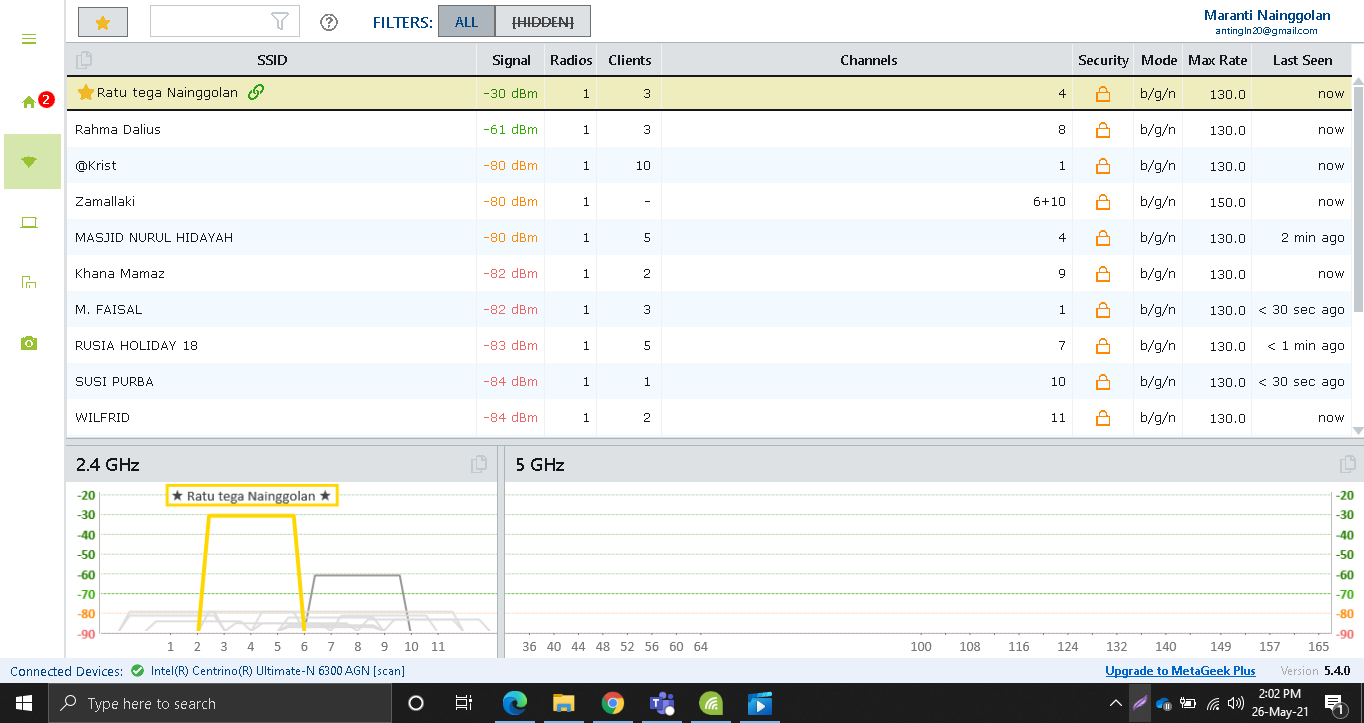
\includegraphics[width=0.4\textwidth]{8.png}
    \caption{Tampilan inSSIDer dalam Rumah}
    \label{tampilan dalam rumah_1}
\end{figure}

\begin{figure}[htbp]
    \centering
    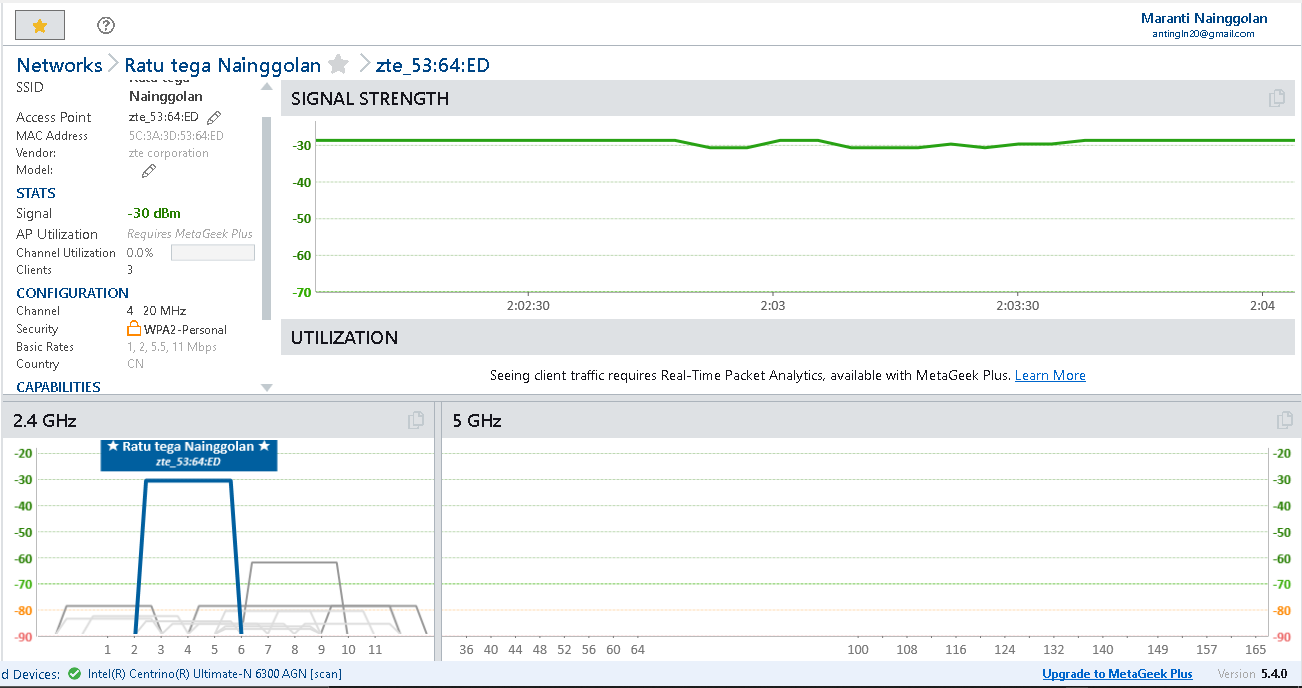
\includegraphics[width=0.4\textwidth]{9.png}
    \caption{Tampilan inSSIDer dalam rumah}
    \label{tampilan dalam rumah_2}
\end{figure}



    \item Pengambilan Data dengan Jarak 15 M dari Rumah

    \begin{figure}[htbp]
        \centering
        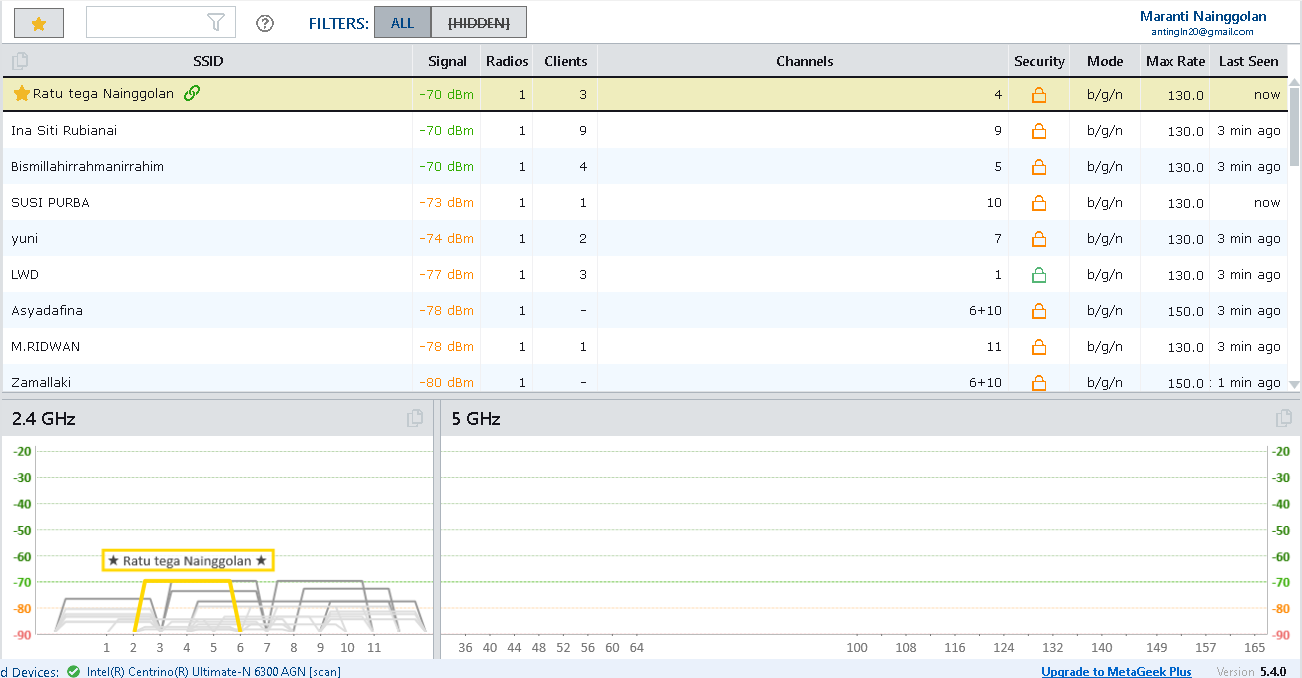
\includegraphics[width=0.4\textwidth]{10.png}
        \caption{Tampilan inSSDer dengan jarak 15 M dari Rumah}
        \label{Tampilan inSSDer dengan jarak 15 M_1}
    \end{figure}

    \begin{figure}[htbp]
        \centering
        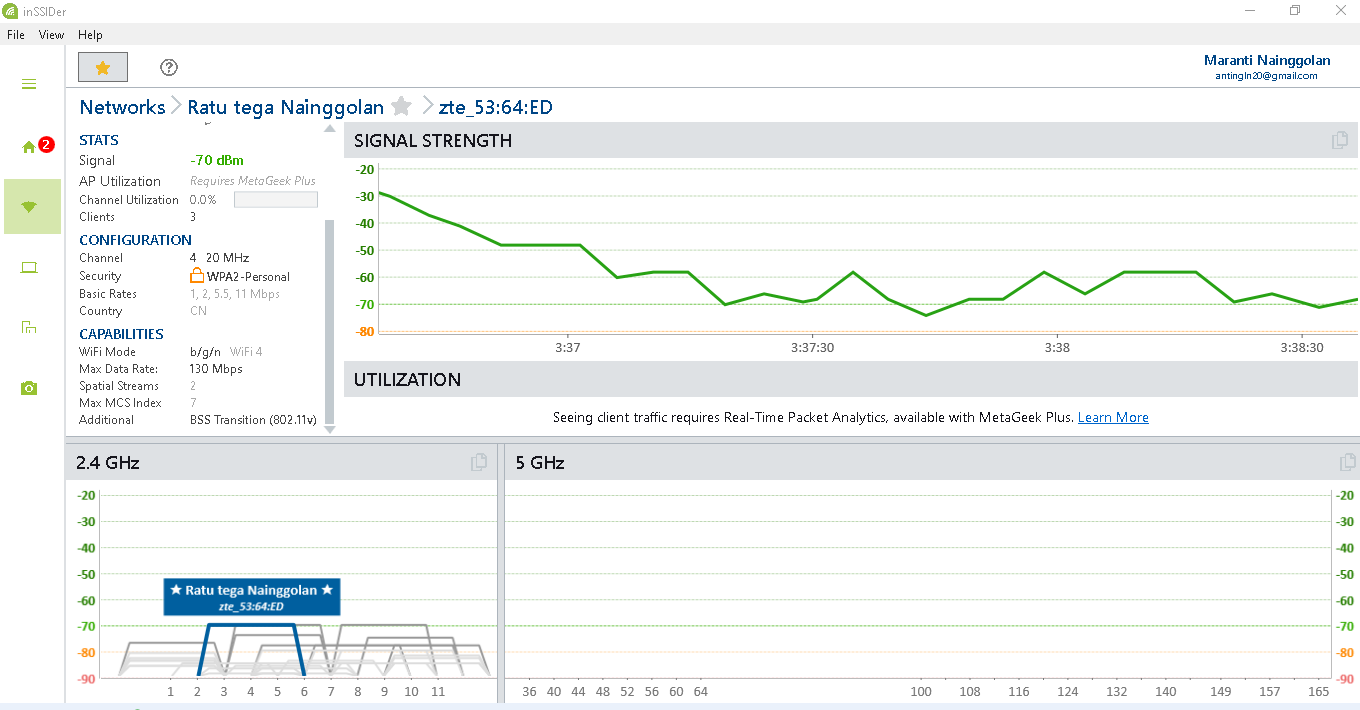
\includegraphics[width=0.4\textwidth]{11.png}
        \caption{Tampilan inSSIDer dengan jarak 15 M dari rumah}
        \label{Tampilan inSSDer dengan jarak 15 M_2}
    \end{figure}

\vspace{0.2cm}

Pada gambar ~\ref{Tampilan inSSDer dengan jarak 15 M_1} dan ~\ref{Tampilan inSSDer dengan jarak 15 M_2}  terlihat bahwa sinyal wireless dengan
SSID ‘Ratu Tega Nainggolan’ memiliki RSSI (Received
Signal Strength Indicator) yakni -70 dBm. Berada
pada kanal 1 dan bekerja pada frekuensi 2,4 GHz. Menggunakan
model WPA-2 personal security dan memiliki
channel 4
\vspace{0.2cm}  

    \item Pengambilan Data dengan Adanya Penghalang / Pembatas (Dinding)~\cite{b6}

    \begin{figure}[htbp]
        \centering
        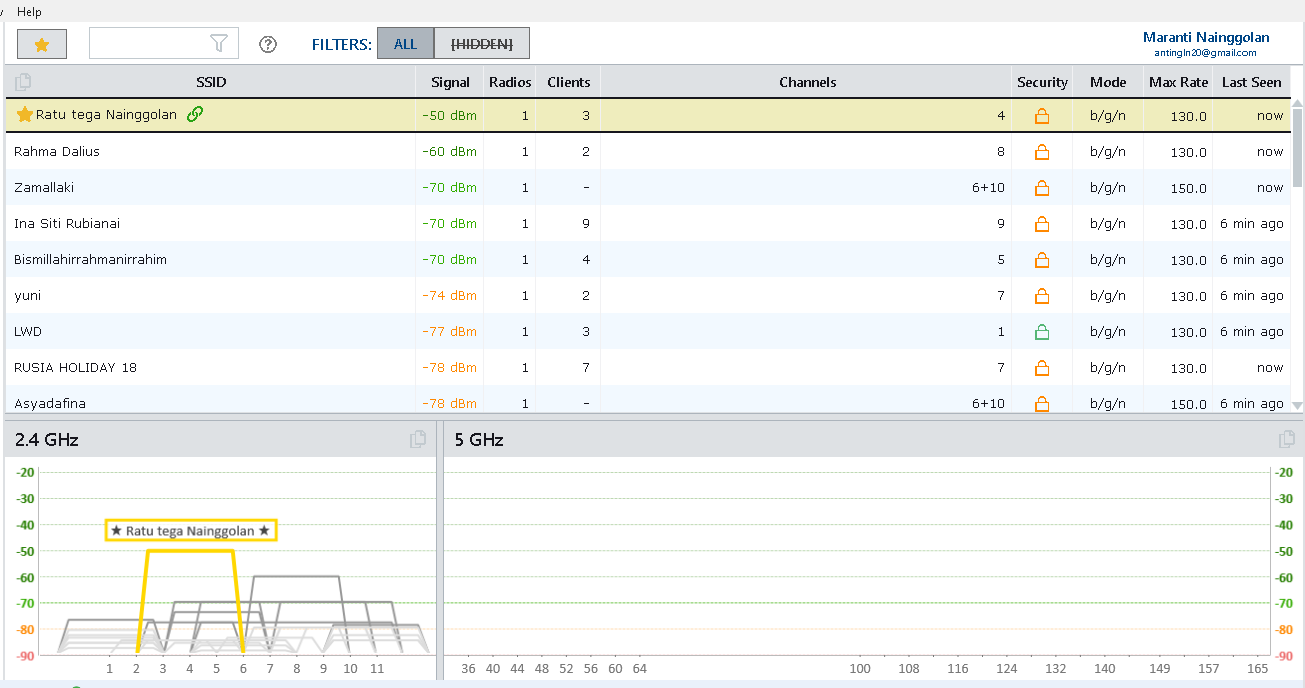
\includegraphics[width=0.4\textwidth]{12.png}
        \caption{Tampilan inSSDer dengan Adanya Pembatas}
        \label{Tampilan dengan Pembatas_1}
    \end{figure}

    \begin{figure}[htbp]
        \centering
        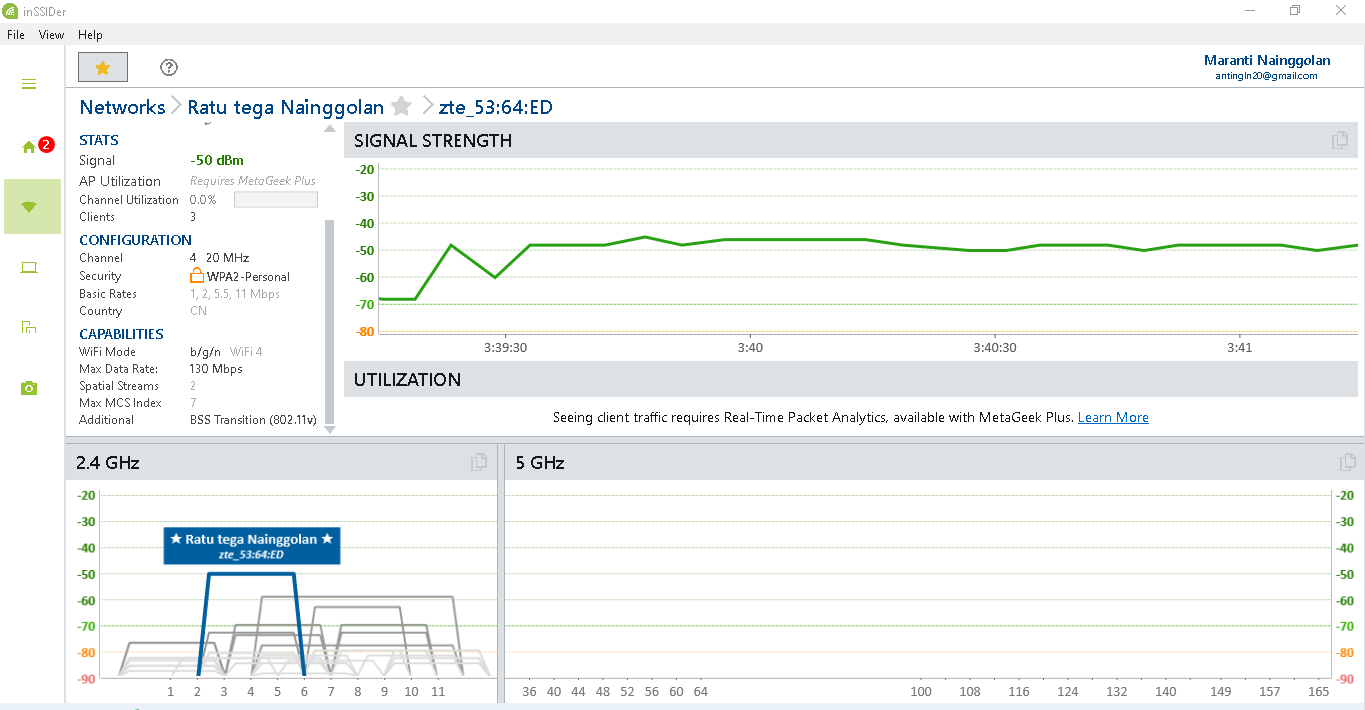
\includegraphics[width=0.4\textwidth]{13.png}
        \caption{Tampilan inSSIDer dengan Adanya pembatas}
        \label{Tampilan dengan Pembatas_2}
    \end{figure}

\vspace{0.2cm}

Pada gambar ~\ref{Tampilan dengan Pembatas_1} dan ~\ref{Tampilan dengan Pembatas_2} terlihat bahwa sinyal wireless
dengan SSID ‘Ratu Tega Nainggolan’ memiliki RSSI (Received Signal Strength Indicator) yakni -50 dBm.
Berada pada kanal 1 dan bekerja pada frekuensi 2,4
GHz. Menggunakan model WPA-2 personal security dan
memiliki channel 4.
\vspace{0.2cm}

    \item Pengambilan Data Saat Berjalan / Mengelilingi Daerah
    Sekitar

\vspace{0.2cm}

Dalam pengambilan kekuatan sinyal wifi saat berjalan,
tentu kekuatan sinyal nya selalu berubah ubah, itu
dikarenan jarak antara pusat wifi dan tempat pengambilan
data, semakin jauh jarak yg ditelusuri maka kekuatan
siyalnya akan terus melemah, begitupun sebaliknya.
\end{itemize}

\vspace{0.2cm}
Dari semua gambar diatas dapat dilihat semua AP menggunakan
atau bekerja di frekuensi 2.4 GHz. Frekuensi
ini memang sering digunakan karena merupakan masuk
dalam standard wireless 802.11b dan 802.11g.Sedangkan
Pada data frekuensi 5 GHz tidak ada AP yang
menggunakannya Terlihat pada panel 5GHz capture
tidak ada SSID yang masuk kategori tersebut.Frekuensi
5GHz ini biasanya digunakan pada 802.11a yang notabennya
memiliki max rate yang sama dengan 802.11g
namun dengan pita yang lebih lebar.


\section{Kesimpulan}
Pengambilan data untuk mengetahui kekuatan sinyal Wi-
Fi dengan menggunakan inSSIDer telah dilakukan dengan
baik. Dari semua gambar diatas dapat dilihat semua AP
menggunakan atau bekerja di frekuensi 2.4 GHz. Frekuensi ini
memang sering digunakan karena masuk dalam standard wireless
802.11b dan 802.11g. Sedangkan Pada data frekuensi 5 GHz tidak ada AP yang menggunakannya Terlihat pada panel
5GHz capture tidak ada SSID yang masuk kategori tersebut.
Frekuensi 5GHz ini biasanya digunakan pada 802.11a yang
notabennya memiliki max rate yang sama dengan 802.11g
namun dengan pita yang lebih lebar.

\begin{thebibliography}{00}
    \bibitem{b1} Pranjal., 2013, Experimental Study of a Wireless Local Area Network, International Journal of Information and Computation Technology, Vol.3 No. 10, pp.1047-1052
    \bibitem{b2} Julia Cynthia Rante, Max Alexander Rura Patras. Analisis Kekuatan Sinyal Vol. 14, No. 1, April 2018: 97-102 ISSN: 1907-0837
    \bibitem{b3} Eka, putra, daniel. 2013. Pengamatan Kuat Sinyal Access Point (AP) Menggunakan inSSIDer
    \bibitem{b4} Kapgate, Y., Vatti, R., Jadhav, S., 2017, WiFi Tools and Signal Strength Analysis, GRD Journals Global Research and Development Journal for Engineering , Vol.2 Issue 10.
    \bibitem{b5} https://www.metageek.com/
    \bibitem{b6} Imansyah2019,Analisis Simulasi Pengaruh Uji Kuat Sinyal Wifi Dari Bahan-Bahan Obstacle,https://scholar.google.co.id/
\bibitem{b7} Rante2018,Analisis Kekuatan Sinyal Wi-Fi Menggunakan Inssider
\end{thebibliography}

\end{document}